\section{第1讲\quad 数值计算}

\item {
    【乘法分配律】
    $(200+2)\times 5 + 5020$
    \ifshowSolution
        \\\fangsong\zihao{5}\textcolor{blue}{
            正解:
            \begin{align*}
                \mbox{原式} &= 200\times 5 + 2\times 5 + 5020 \\
                &= 1000 + 10 + 5020 \\
                &= 6030.
            \end{align*}
        }
    \else
        \vspace{1cm}
    \fi
    % 改. 2025
}

\item {
    【乘法分配律】
    $7\times 19 + 3\times 13\times 41 + 13\times 19$
    \ifshowSolution
        \\\fangsong\zihao{5}\textcolor{blue}{
            正解:
            \begin{align*}
                \mbox{原式} &= (7+13)\times 19 + 39\times 41 \\
                &= 20\times 19 + (40-1)\times (40+1) \\
                &= 380 + 1600 - 1 \\
                &= 1379.
            \end{align*}
        }
    \else
        \vspace{1cm}
    \fi
    % 改. 2021;迎春杯四年级真题.pdf
}

\item {
    【乘法分配律】
    $(18\times 23 - 24\times 17)\div 3 + 5$
    \ifshowSolution
        \\\fangsong\zihao{5}\textcolor{blue}{
            正解:
            \begin{align*}
                \mbox{原式} &= [(17+1)\times (24-1) - 24\times 17]\div 3 + 5 \\
                &= (17\times 24 - 17 + 24 - 1 - 24\times 17)\div 3 + 5 \\
                &= 6\div 3 + 5 \\
                &= 7.
            \end{align*}
        }
    \else
        \vspace{1cm}
    \fi
}

\item {
    【乘法分配律】
    $(11\times 24 - 23\times 9)\div 3 + 3$
    \ifshowSolution
        \\\fangsong\zihao{5}\textcolor{blue}{
            正解:
            \begin{align*}
                \mbox{原式} &= [(9+2)\times (23+1) - 23\times 9]\div 3 + 3 \\
                &= (9\times 23 + 9 + 2\times 23 + 2 - 23\times 9)\div 3 + 3 \\
                &= (9 + 2\times 24)\div 3 + 3 \\
                &= 3 + 16 + 3 \\
                &= 22.
            \end{align*}
        }
    \else
        \vspace{1cm}
    \fi
}

\item {
    【乘法凑十】
    $12\times 25 + 16\times 15$
    \ifshowSolution
        \\\fangsong\zihao{5}\textcolor{blue}{
            正解:
            \begin{align*}
                \mbox{原式} &= 3\times 4\times 25 + 8\times 2 \times 3\times 5 \\
                &= 3\times 100 + 8\times 3\times 10 \\
                &= 300 + 240 \\
                &= 540.
            \end{align*}
        }
    \else
        \vspace{1cm}
    \fi
}

\item {
    【乘法凑十】
    $5\times 432\times 1 - 98 - 7\times 6$
    \ifshowSolution
        \\\fangsong\zihao{5}\textcolor{blue}{
            正解:
            \begin{align*}
                \mbox{原式} &= 5\times 2\times 216 - 98 - 42 \\
                &= 2160 - 140 \\
                &= 2020.
            \end{align*}
        }
    \else
        \vspace{1cm}
    \fi
    %  2020数学花园探秘笔试小中决赛D卷.doc
}

\item {
    【加法凑十】
    $1+3+4+6+7+9+10 + 12$
    \ifshowSolution
        \\\fangsong\zihao{5}\textcolor{blue}{
            正解:
            \begin{align*}
                \mbox{原式} &= (1+9) + (3+7) + (4+6) +10 + 12 \\
                &= 52.
            \end{align*}
        }
    \else
        \vspace{1cm}
    \fi
}

\item {
    【乘法凑十】
    $210\times 6 - 52\times 5$
    \ifshowSolution
        \\\fangsong\zihao{5}\textcolor{blue}{
            正解:
            \begin{align*}
                \mbox{原式} &= 210\times 6 - 26\times 2\times 5 \\
                &= 1000.
            \end{align*}
        }
    \else
        \vspace{1cm}
    \fi
}

\item {
    【尾同头合十】
    $5000- 22\times 82$  
    \ifshowSolution
        \\\fangsong\zihao{5}\textcolor{blue}{
            正解:
            \begin{align*}
                \mbox{原式} &= 5000- 1804 \\
                &= 3196.
            \end{align*}
        }
    \else
        \vspace{1cm}
    \fi
}

\item {
    【乘法分配律】
    $67\times 67 - 34\times 34 + 67 + 34$
    \ifshowSolution
        \\\fangsong\zihao{5}\textcolor{blue}{
            正解:
            \begin{align*}
                \mbox{原式} &= 67\times 68 - 33\times 34 \\
                &= 34\times (134 - 33) \\
                &= 34\times 101 \\
                &= 3434.
            \end{align*}
    }
    \else
        \vspace{1cm}
    \fi
    % 2017年“迎春杯”数学花园探秘科普活动试卷(小中组决赛a卷).doc
}

\item {
    【等差数列求和公式】
    $(1+3+5+\cdots + 89) - (1+2+3+\cdots + 63)$  
    \ifshowSolution
        \\\fangsong\zihao{5}\textcolor{blue}{
            正解:
            \begin{align*}
                \mbox{原式} &= (1+ 89) \times 45 \div 2 - 64\times 63\div 2 \\
                &= 2025 - 2016 \\
                &= 9.
            \end{align*}
        }
    \else
        \vspace{1cm}
    \fi
}

\item {
    【数列】
    数列$1, 1,2,3,5,8\cdots$从第二项起每一项都等于它前面两项之和, 这个数列成为斐波那契数列.其中每一项都叫做斐波那契数.可以证明``任意正整数n都可以成若干个不同的斐波那契数之和'', 那么把100表示成若干个不同的斐波那契数之和有\underline{\hbox to 20mm{}}种表示方法.(只是交换加数的顺序算作同一种)
    \ifshowSolution
        \\\fangsong\zihao{5}\textcolor{blue}{
            正解: 9.
            \begin{align}
                100&=89+3+8\\
                &=89+1+2+8\\
                &=89+1+2+3+5\\
                &=55+34+1+2+3+5\\
                &=55+34+1+2+8\\
                &=55+34+3+8\\
                &=55+13+21+1+2+3+5\\
                &=55+13+21+3+8\\
                &=55+13+21+1+2+8.
            \end{align}
        }
    \else
        \vspace{1cm}
    \fi 
    % 2016年“迎春杯”数学花园探秘初赛试卷(四年级b卷).doc
}

\item {
    【立方和公式】
    $3^3 + 4^3 + 5^3 + 6^3 + 7^3 + 8^3 + 9^3$
    \ifshowSolution
        \\\fangsong\zihao{5}\textcolor{blue}{
            正解:
            \begin{align*}
                \mbox{原式} &= (1^3 + 2^3 + 3^3 + 4^3 + 5^3 + 6^3 + 7^3 + 8^3 + 9^3) - 1^3 - 2^3 \\
                &= (1 + 2 +\cdots + 9)^2 - 9 \\
                &= 45^2 - 9 \\
                &= 2016.
            \end{align*}
        }
    \else
        \vspace{1cm}
    \fi
}

\item {
    【数值计算】
    $99\times 10101\times 111\times 1001001$的末5位数字是多少?
    \ifshowSolution
        \\\fangsong\zihao{5}\textcolor{blue}{
            正解:
            \begin{align*}
                \mbox{原式} &= (1000000-1)\times 111111111 \\
                &= 111111111000000- 111111111 \\
                &= \cdots 88889.
            \end{align*}
        }
    \else
        \vspace{1cm}
    \fi
    % 88889
}

\item {
    【数值计算;数字谜】
    正着读和反着读都一样的数称为回文数, 如121、9889都是回文数, 如果两个回文数的和是 2025, 那么这两个回文数的差是\underline{\hbox to 20mm{}}.
    \ifshowSolution
        \\\fangsong\zihao{5}\textcolor{blue}{
            正解: \\
            (1)判断这两个回文数的长度,可知,至少有一个数为四位.\\
            (2)假设另一个数为一位或两位,分别解相应的数字谜,矛盾,无解.\\
            (3)假设另一个数为三位,解数字谜(相同字母代表相同数字,不同字母的数字可以相同)
            \[
            \begin{array}{l@{\,} c@{\,} c@{\,} c@{\,} c@{\,}}
            & A & B & B & A \\
            + && C  & D & C \\
            \cline{1-5}
            & 2 & 0 & 2 & 5 \\
            \end{array}
            \]
            得$\overline{ABBA}=1551, \overline{CDC}=474, 1551-474=1077.$\\
        }
    \else
        \vspace{1cm}
    \fi
    %    正解: 改  2023;YCB第40届小中组试卷.pdf; 1551+474=2025
}

\item {
    【数字谜】
    下面的算式中, 相同的汉字代表相同的数字, 不同的汉字代表不同的数字, 那么, \\ \myoverline{龙行天下}表示的四位数是\underline{\hbox to 20mm{}}. \\
    \begin{center}
        \myoverline{龙行龘龘} + \myoverlineThree{行天下} = 2024
    \end{center}
    \ifshowSolution 
        \fangsong\zihao{5}\textcolor{blue}{
            正解: \\
            解数字谜:\\
            \[
            \begin{array}{l@{\hspace{1em}} c@{\hspace{1em}} c@{\hspace{1em}} c@{\hspace{1em}} c@{\hspace{1em}}}
            & 龙 & 行 & 龘 & 龘 \\
            + &  & 行 & 天 & 下 \\ 
            \hline
            & 2 & 0 & 2 & 4 \\
            \end{array}
            \]
            \begin{flalign*}
            &(1) 判断进位.十位没有进位,百位有进位.&\\
            &(2) 百位.行=5.&\\
            &(3) 千位.龙=1.&\\
            &(4) 龘=0或2.用枚举法,得龘=0.&\\
            &(5) 天=2,下=4. &
            \end{flalign*}
        }
    \else
        \vspace{1cm}
    \fi
    % 2024
}

\item {
    【数字谜】
    将 $1\sim 9$分别填入到右图的方框中, 每个数字用一次, 使得竖式成立;现在数字 6、7、8已经被填入, 那么竖式的和是\underline{\hbox to 20mm{}}.
    \zihao{3}
    \[
    \begin{array}{l@{\,} c@{\,} c@{\,} c@{\,}}
    & \square & \square & \square \\
    + & \square  & \boxed{7} & \boxed{6} \\
    \cline{1-4}
    & \boxed{8} & \square & \square \\
    \end{array}
    \]
    \ifshowSolution 
        \fangsong\zihao{5}\textcolor{blue}{
            正解: \\
            (1)判断个位.排除 $1+6=7,2+6=8,4+6=10$,还剩$3+6=9,5+6=11$. 如果是$5+6=11$,则十位会产生矛盾.只能是$3+6=9$. \\
            (2)百位.如果没有进位,则与数字不重复矛盾;所以百位两数之和是7. 只能是$2+5=7$.\\
            (3)十位.填入4和1.\\
            \[
            \begin{array}{l@{\,} c@{\,} c@{\,} c@{\,}}
            & \boxed{2} & \boxed{4} & \boxed{3} \\
            + & \boxed{5}  & \boxed{7} & \boxed{6} \\
            \cline{1-4}
            & \boxed{8} & \boxed{1} & \boxed{9} \\
            \end{array}
            \]
        }
    \else
        \vspace{1cm}
    \fi
    % 2023YCB初赛真题答案小中.pdf; 819
    % 改
}

\item {
    【数字谜】
    在下图的加法竖式中, 6个汉字恰好代表6个连续的数字, 那么, ``花园探秘'' 所代表的四位数是\underline{\hbox to 20mm{}}.
    \zihao{3}
    \[
    \begin{array}{l@{\hspace{1em}} c@{\hspace{1em}} c@{\hspace{1em}} c@{\hspace{1em}} c@{\hspace{1em}}}
        & 第 & 3 & 3 & 届 \\
        + & 2 & 0 & 1 & 7 \\ 
        \hline
        & 花 & 园 & 探 & 秘 \\
    \end{array}
    \]
    \ifshowSolution 
        \fangsong\zihao{5}\textcolor{blue}{
            正解: \\
            (1)判断进位.十位没有向前进位,百位没有向前进位. \\
            (2)百位.$园=3$. 因为是6个连续的数字,所以不可能有9.\\
            (3)个位.枚举.如果$届=1$,则$秘=8$,与6个连续数字矛盾;如果$届=2$,则$秘=9$, 矛盾;所以,个位向前进位,$探=5$. 如果$届=4$,则$秘=1$,则这6个连续数字为$0\sim 5$或$1\sim 6$, 都会在千位产生矛盾. \\
            所以,只能$届=7, 秘=4$. \\
            (4)千位.$3\sim 7$共5个数字,其中有数字6.$第=6, 花=8$.
            \[
            \begin{array}{l@{\hspace{1em}} c@{\hspace{1em}} c@{\hspace{1em}} c@{\hspace{1em}} c@{\hspace{1em}}}
                & 6 & 3 & 3 & 7 \\
                + & 2 & 0 & 1 & 7 \\ 
                & \textcircled{0} & \textcircled{0} & \textcircled{1} &  \\ 
                \hline
                & 8 & 3 & 5 & 4 \\
            \end{array}
            \]
        }
    \else
        \vspace{1cm}
    \fi
    % 2021; 8354
}

\item {
    【数字谜】
    在下面的乘法竖式中, 相同的汉字代表相同的数字, 不同的汉字代表不同的数字;那么, \myoverline{迎接夏天} 代表的四位数是\underline{\hbox to 20mm{}}.
    \zihao{3}
    \[
    \begin{array}{l@{\hspace{1em}}  c@{\hspace{1em}} c@{\hspace{1em}} c@{\hspace{1em}}}
        \quad & \quad & 迎 & 春 \\
        \times &\quad & 春 & 天 \\ 
        \hline
        \quad &\quad & 春 & 天 \\ 
        \quad & 晚 & 春 \\ 
        \hline
        迎& 接 & 夏 & 天 \\
    \end{array}
    \]
    \ifshowSolution 
        \fangsong\zihao{5}\textcolor{blue}{
            正解: \\
            (1)黄金三角,$迎=1,晚=9,接=0$.十位没有向前进位,百位没有向前进位. \\
            (2)判断``春''.$春\times 春$的个位是春,则$春=5或6$. \\
            如果$春=5$,则与9矛盾;所以,$春=6$.\\
            (3)判断``夏''.看加法,个位不会向前进位,所以 $夏=2$. \\
            所以,只能$届=7, 秘=4$. \\
            (4)判断``天''.枚举,得 $天=4$.
            \[
            \begin{array}{l@{\hspace{1em}}  c@{\hspace{1em}} c@{\hspace{1em}} c@{\hspace{1em}}}
                \quad & \quad & 1 & 6 \\
                \times &\quad & 6 & 4 \\ 
                \hline
                \quad &\quad & 6 & 4 \\ 
                \quad & 9 & 6 \\
                \hline
                1& 0 & 2 & 4 \\
            \end{array}
            \]
        }
    \else
        \vspace{1cm}
    \fi
    % 2021, 迎春杯四年级真题.pdf; 1024
}

% \item {
%     【数字谜】
%     下列竖式中, 相同汉字表示相同数字, 不同汉字表示不同数字, 且所有汉字对应的数字都不是 0, 2, 5.  ``空歌风度清'' 表示的五位数是\underline{\hbox to 20mm{}}.
%     \zihao{2}
%     \begin{figure}[H] 
%         \centering
%         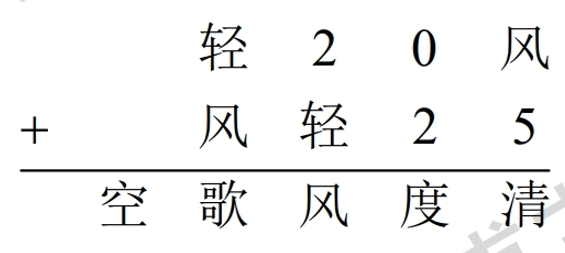
\includegraphics[width=0.4\textwidth]{./pics/Chapter_7/1.png}
%     \end{figure}
%     \vspace{1cm}
%     % 2025数学花园探秘笔试小中年级决赛C卷(B5试卷版).pdf;16934
% }

% \item {
%     $(20+2)\times 5 + 2025$ 
% }


% \item {
%     【乘法分配律】
%     $7\times 17 + 3\times 13\times 43 + 13\times 17$
%     \ifshowSolution
%         \fangsong\zihao{4}
%         \\
%         思路:2021;迎春杯四年级真题.pdf

%         正解: 2017
%     \else
%         \\ \\ \\
%     \fi
% }

% \item {
%     $(9\times 8\times 7 + 6 - 5)\times 4 + 3 -2 +1$
%     \ifshowSolution
%         \fangsong\zihao{4}
%         \\
%         思路: 迎春杯四年级2022-试卷.pdf

%         正解: 2022
%     \else
%         \\ \\ \\
%     \fi
% }

% \item {
%     【数值计算;数字谜】有一些自然数, 如 121 和 2552, 从左到右和从右到左的数字顺序相同, 我们把这样的自然数叫做``回文数''. 已知两个回文数的和是 2022, 则这两个回文数的差是\underline{\hbox to 20mm{}}.
%     \vspace{1cm}
%     % 正解:  迎春杯三年级2022-试卷.pdf; 1740
% }